\documentclass[conference]{IEEEtran}
\usepackage{graphicx}
\usepackage{booktabs}
\usepackage{array}
\usepackage{url}
\usepackage[hidelinks]{hyperref}
\usepackage{listings}
\lstset{basicstyle=\ttfamily\footnotesize,columns=fullflexible,breaklines=true,frame=single,xleftmargin=2pt,xrightmargin=2pt}
\graphicspath{{./}{../}{../../../docs/}}
\makeatletter\g@addto@macro{\UrlBreaks}{\do\-\do\_}\makeatother
\newcommand{\cmd}[1]{\texttt{#1}}
\newcommand{\src}[1]{\\\footnotesize\textit{Source:} \nolinkurl{evidence/Phase-2/#1}}
\newcommand{\srcp}[1]{\\\footnotesize\textit{Source:} \nolinkurl{#1}}

\begin{document}

\title{Hardening a Two-Host Private Service Network:\\ Backup DNS, TTL-Driven Change, Service Isolation, Failover and Edge Cutover}

\author{\IEEEauthorblockN{Yatin Singh}
\IEEEauthorblockA{\textit{B.Tech CS \& AI}\\
\textit{Newton School of Technology}\\
\textit{Rishihood University}}
\and
\IEEEauthorblockN{Dadi Dinesh}
\IEEEauthorblockA{\textit{B.Tech CS \& AI}\\
\textit{Newton School of Technology}\\
\textit{Rishihood University}}}

\maketitle

\begin{abstract}
This report describes Phase~2 of a Computer Networks course project in which a private service network was built by hand on two macOS laptops sharing one Wi-Fi hotspot. In Phase~1 a client resolved the private name \cmd{app.team1.test} through our own dnsmasq resolver, connected over HTTPS to an nginx edge that terminates TLS with a locally issued certificate, and was load-balanced across two Express backends. Phase~2 extends this network with five resilience mechanisms: a backup DNS resolver, a record change governed by a 30-second TTL, packet-filter isolation of the backend ports, passive health-check failover in nginx, and a DNS-based migration to a standby edge. Each mechanism was demonstrated with a before/after test whose screenshot is referenced in the text. We also report the faults met while running the tests and the layer-by-layer method used to diagnose them. All five mechanisms behaved as intended; the server host remains the single point of failure of the design.
\end{abstract}

\begin{IEEEkeywords}
DNS, TTL, dnsmasq, nginx, failover, reverse proxy, TLS termination, packet filter, troubleshooting
\end{IEEEkeywords}

\section{Introduction}
A request to a web service crosses several independent layers: name resolution, IP reachability, a TCP connection, a TLS handshake and the HTTP exchange. Phase~1 of the project built each layer on two laptops and captured it with Wireshark. Phase~2 asks what happens when part of the system fails or must change, and how the network can be made to tolerate it.

The brief defines six extensions: (A) a backup DNS resolver, (B) TTL and a controlled record change, (C) isolation of the backend services, (D) high-availability failover, (E) a DNS-based edge migration and (F) a troubleshooting challenge injected by the faculty. Sections~\ref{sec:a}--\ref{sec:e} document the design, test and result of A--E. Extension~F is evaluated live; Section~\ref{sec:trouble} describes the faults we diagnosed while running the tests and the method we use for it.

\section{System Architecture}
\subsection{Machines and Roles}
The team has two members and two laptops, and the brief allows teams of two or three to combine machine roles. Table~\ref{tab:roles} lists the roles; Fig.~\ref{fig:topo} shows the Phase~1 topology on which Phase~2 builds. Mac~1 is a college-managed laptop whose firewall blocks incoming LAN connections and cannot be changed by the user, as established with \cmd{tcpdump} in Phase~1. It therefore acts as the client, and every LAN-facing server runs on Mac~2. In the Phase~2 session the hotspot assigned Mac~2 the address 10.68.13.178.

\begin{table}[htbp]
\caption{Machine Roles and Services}
\label{tab:roles}
\centering
\begin{tabular}{@{}l l l@{}}
\toprule
Host & Role & Service / port \\
\midrule
Mac 1 & Client & browser, curl, dig \\
Mac 2 & Primary DNS & dnsmasq, UDP 53 \\
Mac 2 & Primary edge & nginx, TCP 443 (80 $\rightarrow$ 301) \\
Mac 2 & Backend A / B & Express, TCP 4000 / 6000 \\
\midrule
\multicolumn{3}{@{}l@{}}{\textit{Added in Phase 2:}}\\
Mac 1 & Backup DNS & dnsmasq, 127.0.0.1:53 \\
Mac 1 & Standby edge & nginx, 127.0.0.1:443 \\
Mac 2 & Isolation & pf rule on \cmd{en0} \\
\bottomrule
\end{tabular}
\end{table}

\begin{figure}[htbp]
\centerline{\includegraphics[width=\columnwidth]{topology.png}}
\caption{Phase~1 topology and request flow on which the Phase~2 extensions are built.\srcp{docs/topology.png}}
\label{fig:topo}
\end{figure}

\subsection{Why Two Services Run on the Client's Loopback}
Because Mac~1 cannot accept LAN connections, the backup resolver (A) and the standby edge (E) listen on Mac~1's loopback address and serve Mac~1 itself, which is the client in every test. The mechanisms under test---falling back to a second resolver, and moving traffic to a different edge when a DNS record changes---behave exactly as they would on a separate host; only their reach is limited to one client.

\section{Backup DNS Resolver (Extension A)}\label{sec:a}
\textit{Design.} A second dnsmasq~\cite{dnsmasq} instance on Mac~1 listens on 127.0.0.1 and carries the same \cmd{address=} records as the primary, both pointing to Mac~2:
\begin{lstlisting}
listen-address=127.0.0.1
bind-interfaces
no-resolv
server=8.8.8.8
local=/team1.test/
address=/app.team1.test/10.68.13.178
address=/api.team1.test/10.68.13.178
local-ttl=30
\end{lstlisting}
Mac~1's resolver list was set to the primary (Mac~2) followed by the backup (127.0.0.1).

\textit{Test.} The primary was stopped on Mac~2 (\cmd{brew services stop dnsmasq}) and Mac~1's resolver was set to the backup alone.

\textit{Result.} Fig.~\ref{fig:a} shows \cmd{dig app.team1.test} on Mac~1 returning \cmd{NOERROR}, the authoritative flag and \cmd{app.team1.test 30 IN A 10.68.13.178}, answered by \cmd{SERVER: 127.0.0.1\#53}, and \cmd{curl https://app.team1.test} still returning \cmd{hello from backend B}. Name resolution and the service survived the loss of the primary resolver.

\textit{DNS failure versus application failure.} When DNS fails, the client cannot obtain an address and never contacts the server; the symptom is NXDOMAIN or a resolver timeout. When the application fails, resolution succeeds and the server answers with an error, such as nginx's \cmd{502 Bad Gateway} when no backend is available (Phase~1).

\begin{figure}[htbp]
\centerline{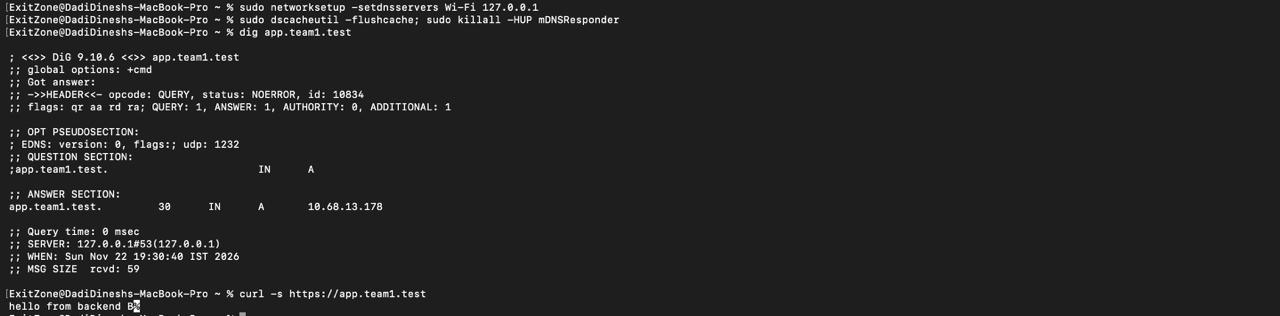
\includegraphics[width=\columnwidth]{A-backup-works.jpeg}}
\caption{With the primary resolver stopped, Mac~1 resolves the name through its backup resolver on 127.0.0.1 and the site still responds.\src{A-backup-works.jpeg}}
\label{fig:a}
\end{figure}

\section{TTL and Controlled Record Change (Extension B)}
\textit{Design.} The project records carry \cmd{local-ttl=30}, so a resolver or client may cache each answer for 30 seconds~\cite{rfc1034}.

\textit{Test.} The name was looked up on Mac~1 with \cmd{dscacheutil}, which reads the operating-system resolver cache. The record on Mac~2 was then changed to 10.10.10.10 and dnsmasq restarted, and the lookup was repeated every ten seconds with a timestamp. Finally the record was restored and the client cache was flushed.

\textit{Result.} After the change, Mac~1 kept returning the cached address 10.68.13.178 (Fig.~\ref{fig:b}, top) until the 30-second TTL expired; the screenshot captures this cached phase. After the record was restored, flushing the cache with \cmd{dscacheutil -flushcache} and \cmd{killall -HUP mDNSResponder} returned the correct address immediately (Fig.~\ref{fig:b}, bottom). \cmd{dig} is unsuitable for showing this effect because it queries the server directly and bypasses the client cache.

\textit{Production relevance.} Before a migration, operators lower the TTL so that a record change propagates in seconds instead of hours, and keep the old target running until cached answers have expired.

\begin{figure}[htbp]
\centering
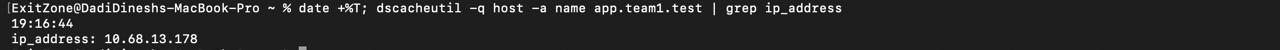
\includegraphics[width=\columnwidth]{B-ttl.jpeg}\\[3pt]
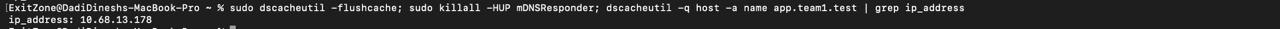
\includegraphics[width=\columnwidth]{B-flush.jpeg}
\caption{Top: a timestamped lookup through the OS cache returns the cached address. Bottom: after a manual cache flush the lookup returns the correct record at once.\src{B-ttl.jpeg, B-flush.jpeg}}
\label{fig:b}
\end{figure}

\section{Service Isolation (Extension C)}
\textit{Design.} In Phase~1 the backends listened on all interfaces, so a client could bypass the edge and reach them directly. We added a pf~\cite{pf} rule on Mac~2, after backing up \cmd{/etc/pf.conf}:
\begin{lstlisting}
set skip on lo0
block drop in quick on en0 proto tcp \
      from any to any port { 4000 6000 }
pass all
\end{lstlisting}
The rule drops any connection to the backend ports arriving on the Wi-Fi interface, while loopback traffic---which nginx uses to reach the backends---is not filtered.

\textit{Result.} Before the rule, \cmd{curl http://<Mac 2>:4000} from Mac~1 reached Backend~A directly (Fig.~\ref{fig:c}, top). With the rule loaded (Fig.~\ref{fig:c}, middle), the same request timed out after 3~s, while \cmd{https://app.team1.test} still returned \cmd{hello from backend A} through nginx (Fig.~\ref{fig:c}, bottom). Clients can now reach the backends only through the edge.

\textit{Rollback.} \cmd{pfctl -f /etc/pf.conf} reloaded the original ruleset; Fig.~\ref{fig:crb} shows only the system's \cmd{com.apple} anchors remaining. pf had been enabled by macOS before the demonstration, so it was left enabled. Our backend ports are 4000 and 6000 rather than the brief's 3001 and 3002; the isolation logic is unchanged.

\begin{figure}[htbp]
\centering
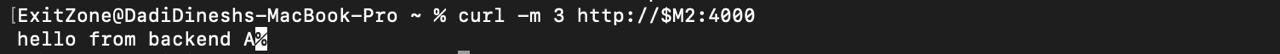
\includegraphics[width=\columnwidth]{C-before.jpeg}\\[3pt]
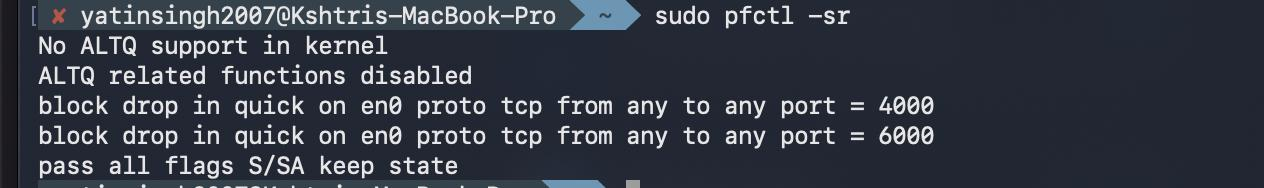
\includegraphics[width=\columnwidth]{C-rules.jpeg}\\[3pt]
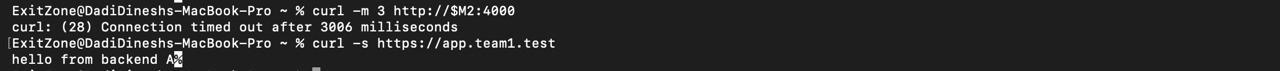
\includegraphics[width=\columnwidth]{C-after.jpeg}
\caption{Top: direct access to Backend A from Mac~1 before isolation. Middle: the pf rules loaded on Mac~2. Bottom: direct access times out while access through the edge still works.\src{C-before.jpeg, C-rules.jpeg, C-after.jpeg}}
\label{fig:c}
\end{figure}

\begin{figure}[htbp]
\centerline{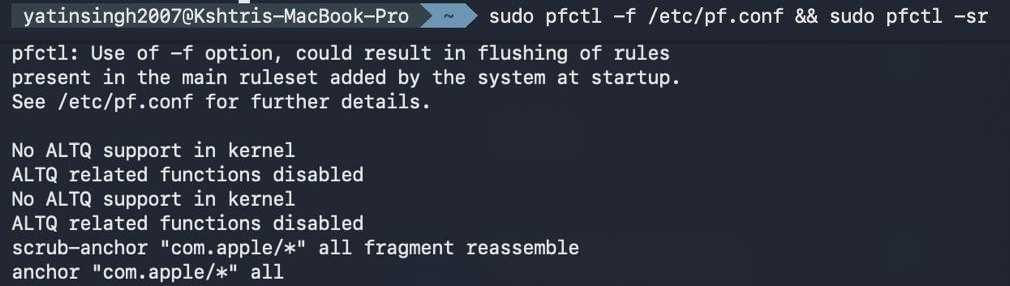
\includegraphics[width=0.9\columnwidth]{C-rollback-crop.png}}
\caption{Rollback: the original ruleset (system anchors only) is restored.\src{C-rollback.jpeg (cropped)}}
\label{fig:crb}
\end{figure}

\section{High-Availability Failover (Extension D)}
\textit{Design.} Each upstream server is declared with \cmd{max\_fails=1 fail\_timeout=10s}, and \cmd{proxy\_next\_upstream error timeout http\_502 http\_503} lets nginx retry a failed attempt on the other server~\cite{nginxup}. This is passive health checking: a backend is marked unavailable after a real request to it fails, and is retried after \cmd{fail\_timeout}.

\textit{Test and result.} With both backends running, requests from Mac~1 were served by both Backend~A and Backend~B (Fig.~\ref{fig:d}, top). With Backend~A stopped, all six requests were served by Backend~B and none failed (Fig.~\ref{fig:d}, bottom): nginx retried the failed attempt on B and stopped sending traffic to A. After Backend~A was restarted and \cmd{fail\_timeout} elapsed, requests were again spread across both backends (observed live; no screenshot was taken of this step).

\textit{Single point of failure.} Mac~2 hosts the primary resolver, the primary edge and both backends; if it fails, the service is lost. Removing this requires a second edge on another host sharing a floating virtual IP (for example VRRP with keepalived) or DNS failover across two edges, and backends on separate hosts.

\begin{figure}[htbp]
\centering
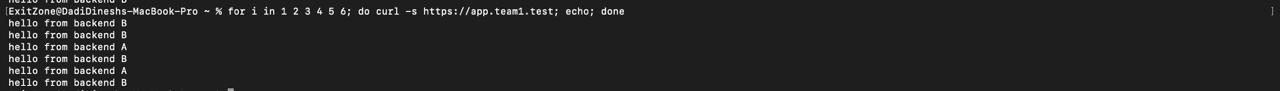
\includegraphics[width=\columnwidth]{D-before.jpeg}\\[3pt]
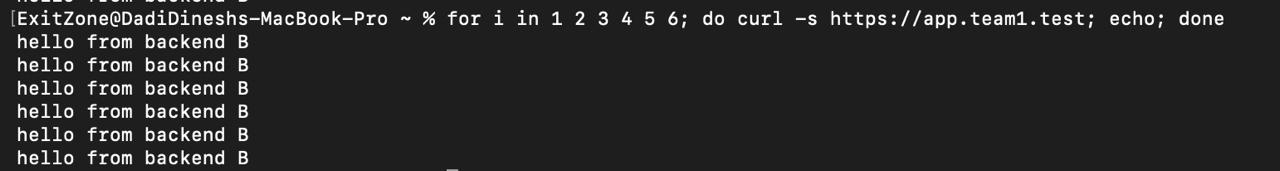
\includegraphics[width=\columnwidth]{D-a-down.jpeg}
\caption{Top: requests served by both backends. Bottom: with Backend A stopped, every request is served by Backend B without errors.\src{D-before.jpeg, D-a-down.jpeg}}
\label{fig:d}
\end{figure}

\section{DNS-Based Edge Cutover (Extension E)}\label{sec:e}
\textit{Design.} A standby nginx on Mac~1 serves the same certificate for \cmd{app.team1.test} and proxies to the same two backends. Each edge adds a response header identifying itself: \cmd{X-Edge: mac2} on the primary and \cmd{X-Edge: mac1} on the standby. Before the cutover, the standby was tested directly with \cmd{curl --resolve app.team1.test:443:127.0.0.1}, which returned \cmd{X-Edge: mac1} and a backend response (Fig.~\ref{fig:e}, top).

\textit{Test.} A loop on Mac~1 printed the time and requested \cmd{https://app.team1.test} every five seconds, printing the \cmd{X-Edge} header. On Mac~2, the \cmd{app.team1.test} record was changed to point to the standby edge and dnsmasq was restarted.

\textit{Result.} Requests kept reaching \cmd{mac2} while the client held the cached answer and switched to \cmd{mac1} between 19:58:19 and 19:58:25 (Fig.~\ref{fig:e}, bottom), consistent with the 30-second TTL. No request failed and no certificate warning appeared, because both edges present the same certificate for the same name~\cite{rfc8446}. The record was then restored to Mac~2 and the standby stopped.

\begin{figure}[htbp]
\centering
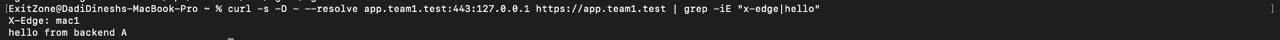
\includegraphics[width=\columnwidth]{E-standby-ready.jpeg}\\[4pt]
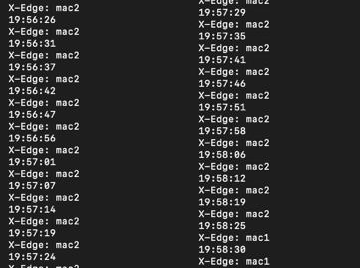
\includegraphics[width=0.75\columnwidth]{E-cutover-crop.png}
\caption{Top: the standby edge answers with \cmd{X-Edge: mac1}. Bottom: the cutover log (left column continues on the right); responses move from \cmd{mac2} to \cmd{mac1} once the cached record expires.\src{E-standby-ready.jpeg, e-cutover.jpeg (rearranged)}}
\label{fig:e}
\end{figure}

\section{Troubleshooting Findings}\label{sec:trouble}
Table~\ref{tab:faults} lists the faults met while running the tests. All of them looked like ``the site does not load'', yet each had a different cause, and four of the five were at the DNS layer.

\begin{table*}[htbp]
\caption{Faults Encountered During Phase 2 and Their Diagnosis}
\label{tab:faults}
\centering
\begin{tabular}{@{}>{\raggedright}p{4.2cm} l >{\raggedright}p{5.6cm} >{\raggedright\arraybackslash}p{4.6cm}@{}}
\toprule
Symptom & Layer & Cause & Fix \\
\midrule
curl printed \cmd{dns:0 connect:0}; \cmd{curl -v} showed a resolver timeout & DNS & Name resolution failed before any connection was attempted & Queried each resolver with \cmd{dig @server} to find the faulty one \\
Queries to Mac 2 timed out & IP / DNS & The hotspot had assigned a new subnet; dnsmasq was still configured for the old address & Rewrote \cmd{listen-address} and the records with the current IP \\
Port 53 on Mac 2 held by Cloudflare WARP & DNS & WARP's DNS proxy was running and dnsmasq was not & Disconnected WARP, restarted dnsmasq, checked \cmd{lsof -iUDP:53} \\
Backup resolver never answered & DNS & Its config contained a literal placeholder instead of an IP, so dnsmasq failed to start & Rewrote the config with the real address \\
Plain \cmd{dig} silent while \cmd{dig @127.0.0.1} answered & DNS & The resolver list had just changed and the backup was not yet running correctly & Restarted the backup, flushed the cache, queried it explicitly \\
\bottomrule
\end{tabular}
\end{table*}

The method we use for these faults and for Extension~F checks one layer at a time, bottom-up: name resolution (\cmd{dig}), IP reachability (\cmd{ping}), TCP (\cmd{nc -vz host 443}), TLS (\cmd{openssl s\_client}), HTTP (\cmd{curl -v}) and finally the nginx error log, which names a failing upstream. A \cmd{502} at the HTTP step points to the backends, not the network.

\section{Discussion}
The extensions fall into three groups. A, D and E add redundancy, but each moves the single point of failure rather than removing it: the backup resolver and the standby edge share a host with the client, and the primary edge shares a host with every backend. B and E show that DNS-based traffic management is bounded by caching; the TTL is a trade-off between query load and how quickly a change takes effect, and E's cutover completed only after cached answers expired. C shows that placing services behind a reverse proxy is not isolation by itself; the backend ports must also be closed on the network interface. The main practical constraint was the managed client laptop, which could host services only on its loopback; with a third, unmanaged host, the backup resolver and the standby edge would serve every client on the LAN.

\section{Conclusion}
Building on the Phase~1 network, we demonstrated a backup resolver that keeps names resolvable when the primary stops, TTL-governed propagation of a record change, firewall isolation that leaves only the edge able to reach the backends, automatic failover in nginx, and a DNS-based migration to a standby edge without failed requests or certificate warnings. The remaining single point of failure is the server host, which two edges sharing a floating virtual IP, with backends on separate machines, would remove.

\section*{Learning Summary}
\textit{A, Backup DNS.} A second resolver keeps names working only if clients list it; a DNS outage (no address) looks different from an application outage (an address that returns an error).

\textit{B, TTL.} The TTL decides how long a change takes to reach clients; operators lower it before migrations and keep old targets alive until caches expire.

\textit{C, Isolation.} A firewall rule that blocks backend ports on the LAN but skips loopback enforces edge-only access; backing up the original rules made the change safe to undo.

\textit{D, Failover.} Passive health checks hide a backend failure from users and restore balancing automatically, but redundant backends do not remove the edge host as a single point of failure.

\textit{E, Edge cutover.} DNS can move traffic to a new edge without touching clients, but only after cached answers expire, so both edges must stay up during the switch; a shared certificate keeps the change invisible at the TLS layer.

\textit{F, Troubleshooting.} Checking layers in order---DNS, IP, TCP, TLS, HTTP---found every fault quickly and avoided changing parts that were already working.

\begin{thebibliography}{00}
\bibitem{rfc1034} P. Mockapetris, ``Domain names---concepts and facilities,'' RFC 1034, IETF, Nov. 1987.
\bibitem{rfc8446} E. Rescorla, ``The Transport Layer Security (TLS) protocol version 1.3,'' RFC 8446, IETF, Aug. 2018.
\bibitem{nginxup} NGINX, ``Module ngx\_http\_upstream\_module,'' nginx documentation. [Online]. Available: \url{https://nginx.org/en/docs/http/ngx_http_upstream_module.html}
\bibitem{dnsmasq} S. Kelley, ``dnsmasq,'' manual page. [Online]. Available: \url{https://thekelleys.org.uk/dnsmasq/docs/dnsmasq-man.html}
\bibitem{pf} OpenBSD, ``pf.conf---packet filter configuration file,'' manual page. [Online]. Available: \url{https://man.openbsd.org/pf.conf}
\end{thebibliography}

\end{document}
